\section{Gravitational waves and their detection}

In 1893, Oliver Heaviside wrote about attempting to localise gravity in a similar manner to the work of Maxwell in which gravity may move as a wave and propagate at the speed of light \cite{Heaside1894}. After Einstein published his general theory of relativity, he theorised that the equations would produce gravitational waves. Einstein mentions, in a letter to Schwarzchild, gravitational waves are not produced by dipole interaction like electromagnetic waves thus has no equivalent negative charge \cite{universe2030022}. 

Rainer Weiss is credited as ``pioneer[ing] the concept of using lasers for an interferometric gravitational wave detector" \cite{noauthor_rainer_2024}. Weiss co-founded the LIGO project and was credited to the design of the kilometre long Michelson interferometer, the design pictured in Figure \ref{fig:GWobservatory}. This detector consists of a laser beam that is split into two perpendicular arms using a beam splitter, down each arm is a mirror where the laser beam is then recombined at the splitter and interfere with each other creating an interference pattern. When a GW passes through the detector, it alternately stretches and compresses spacetime in the detectors. This results in one arm of the interferometer will get slightly longer while the other stays slightly shorter, and vice versa. The changes in arm length are incredibly small, on the order of a fraction of the width of a proton $(10^{-18}\space m)$.

Detecting such tiny changes requires isolating the interferometer from external perturbations (e.g. seismic activity, and thermal fluctuations). Various techniques are used to remove as much background noise as possible but it is not immune to all changes in its environment. False positives from a detector may occur due to external factors, these may be mislabelled as a detection of a GW. However, through a network of gravitational wave detectors across the globe these false positives can be filtered out.

In 2017, almost two years after the first observation of gravitational waves, the GW170817 event was detected by the LIGO detectors \cite{Cannon_2012}, produced by the in-spiral of a binary pair of neutron stars. Initially detected by the two LIGO detectors (Livingston and Hanford), it was only until visual inspection of the LIGO data showed the signs of the observation of GWs \cite{Abbott_2017}. The detection was not as clear on the Virgo detector due to its lower sensitivity, demonstrated in Figure \ref{fig:GW170817}, but this lead to helping the localisation of the source since it was implied that it was located within one of Virgos blind spot. With the aid of the three GW detectors a location of the source was able to be derived in the sky \cite{PhysRevLett.119.161101}. In addition, the detection of GW170817 allowed for a direct measurement of the Hubble constant by combining the distance from gravitational waves with the redshift from electromagnetic observations, providing a new and independent way to measure the expansion rate of the Universe \cite{Abbott2017}.

\begin{figure}[h!]
    \centering
    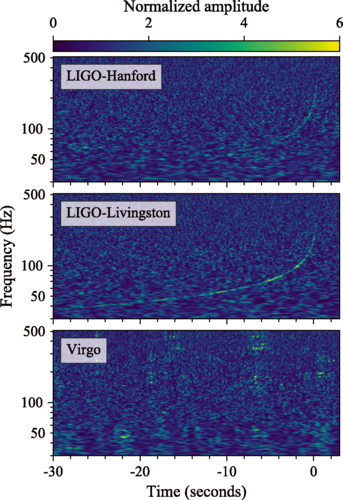
\includegraphics[width=0.4\linewidth]{images/medium.png}
    \caption{GW170817 event observed by the LIGO-Hanford (top), LIGO-Livingston(middle), and Virgo(bottom detectors). The LIGO detectors observing clearly the event, with the Virgo detector unable to resolve the event. \cite{Abbott_2017}}
    \label{fig:GW170817}
\end{figure}


\begin{figure}[h!]
\caption{A diagram depicting the basic operations of a GW observatory \cite{noauthor_ligo_2025} \textbf{1} shows the detector in normal operation where the beams will produce an interference pattern on the right hand side of the diagram. \textbf{2} Depicts a GW passing over the detector in turn this will change the path length of the beam down on left hand side and thus will change the interference pattern on the right.
\label{fig:GWobservatory}}
{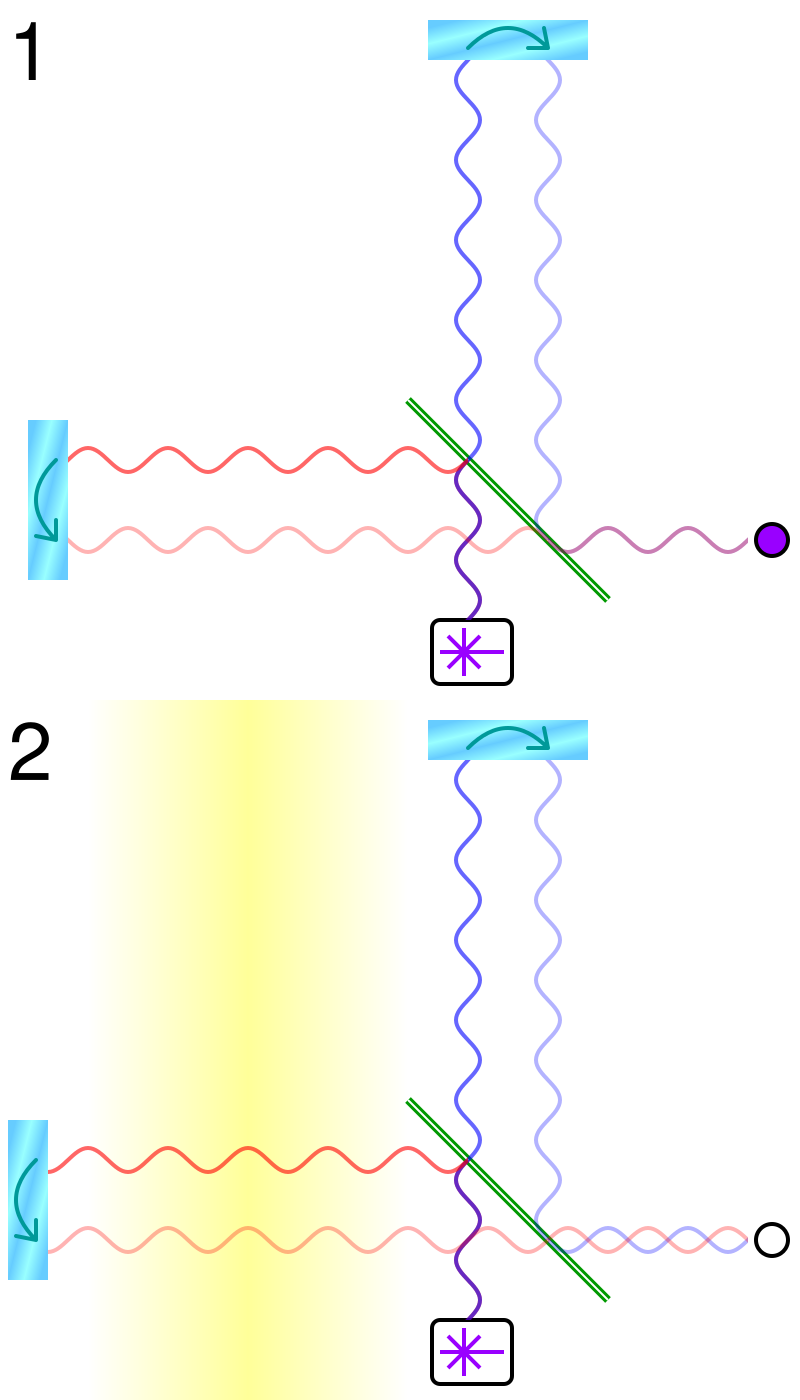
\includegraphics[width=0.3\textwidth]{images/Gravitational_wave_observatory_principle.png}}
\end{figure}

\section{Aims and motivations}

The motivation behind this project is to intuitively demonstrate how we detect GWs on earth from an array of multiple GW detectors at different locations across the globe. Using water as a medium for propagating waves in, where the movement of a bob on top of the surface of the water is detected through a camera and interpreted by a machine learning algorithm simulates a GW detector. The project is aimed at being capable of being replicated by anyone, engaging the public in a practical manor such as a science festival. Using some household items and a laptop to allow the public to explore the side of experimental physics and become interested in astrophysics. 

From conception the projects design was to be simple and easily reproducible with that in mind. This report will demonstrate how the detector was developed, how it can be used and the results that can be expected when reproducing the experiment. All in an effort to clarify how we detect one of the most discussed phenomena of the twenty-first century.